\documentclass{standalone}

\usepackage{TikzStyle}
\usepackage{mystyle}

% pos, num
\newcommand{\Cell}[2]{%
    \draw[xshift=#1 cm,very thick] (0,0) -- (0,-1);
    \node () at ([shift={(#1,0)}]0.7,-0.5) {$\textit{nome}_{#2}$};
    \draw[xshift=#1 cm] (1.5,0) -- (1.5,-1);
    \node () at ([shift={(#1,0)}]2.3,-0.5) {$\textit{valore}_{#2}$};
    \draw[xshift=#1 cm,very thick] (3,0) -- (3,-1);
}

\newcommand{\gpoint}[2]{%
\filldraw [gray] (#1,#2) circle [radius=2pt]
}

\begin{document}
    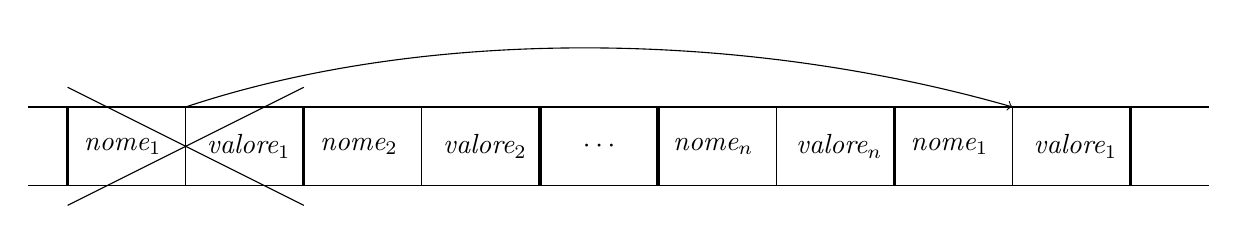
\begin{tikzpicture}
        \draw (0,0) -- (15,0);
        \draw (0,-1) -- (15,-1);
        \Cell{0.5}{1};
        \Cell{3.5}{2};
        \Cell{8}{n};
        \Cell{11}{1};
        \draw (0.5,0.25) -- (3.5,-1.25);
        \draw (0.5,-1.25) -- (3.5,0.25);
        \node () at (7.25,-0.5) {$\cdots$};
        \draw[->] (2,0) .. controls (5,1) and (9,1) .. (12.5,0);
    \end{tikzpicture}
\end{document}
